\begin{figure}[tb]
    \vspace{-2mm}

    \centering
    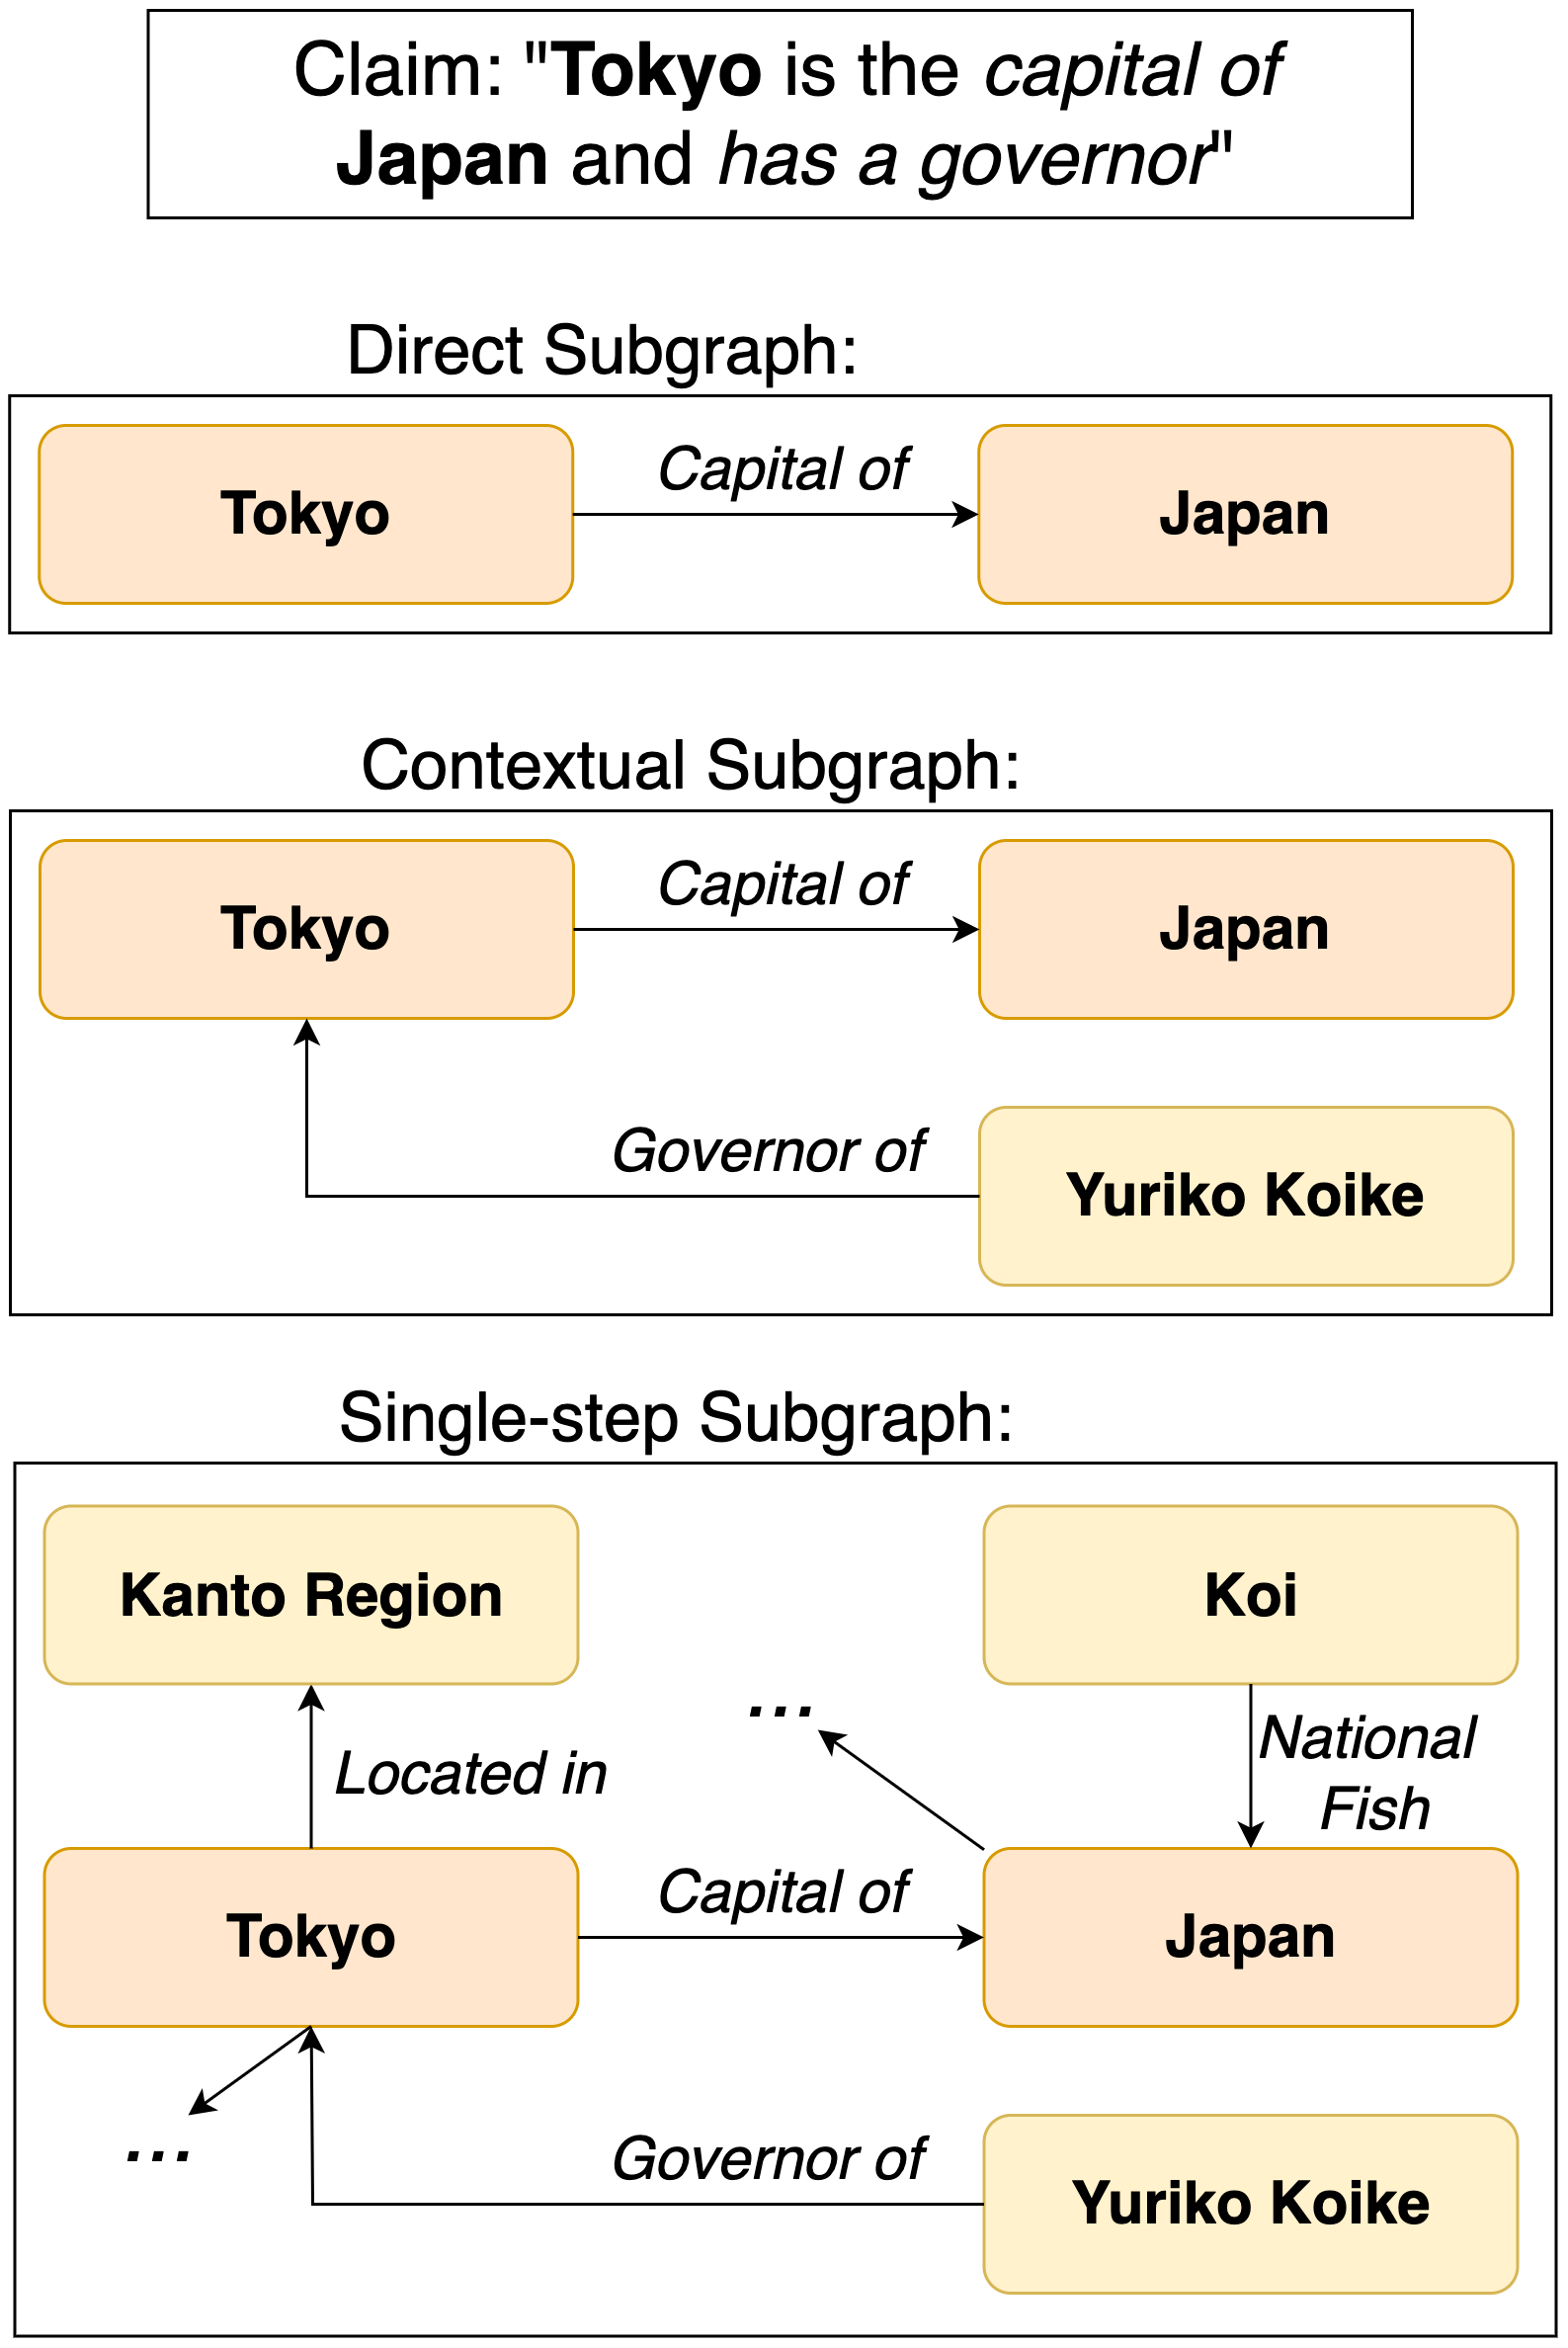
\includegraphics[width=0.47\textwidth]{figures/raw_figures/subgraph_types.png}

    \caption{\textbf{Examples of the different subgraphs explored in this article}. Boxes and \textbf{bold letters} represent entities, while arrows and \textit{italic letters} represent relations. This claim is meant for illustrative purposes and is not present in the \textsc{FactKG} dataset.}

\label{fig:subgraph_types}
\end{figure}

